\chapter{Used Components}\label{ch:usedComponents}
\section{Sensors}\label{sec:sensors}
\subsection{Thermal Camera}\label{ssec:HWthermalCamera}

\begin{table}[h]
    \begin{tabular}{ll}
        Optical resolution & 382 $\times$ 288 \\ \midrule
        Detector & FPA, uncooled \SI{17}{\micro\meter} $\times$ \SI{17}{\micro\meter} \\ \midrule
        Spectral range &  \SI{8}{\micro\meter} $-$ \SI{14}{\micro\meter} \\ \midrule
        Temperature ranges & 
        \begin{tabular}{@{}l@{}}\SI{-20}{\celsius} $-$ \SI{100}{\celsius}\\
            \SI{0}{\celsius} $-$ \SI{250}{\celsius} \\
            \SI{150}{\celsius}$-$ \SI{900}{\celsius}
        \end{tabular} \\ \midrule
        Frame rate & \SI{80}{\hertz} \\ \midrule
        Thermal sensitivity (NETD) &
        \begin{tabular}{@{}l@{}}
            \SI{75}{\milli\kelvin} with \SI{29}{\degree} x \SI{}{\degree} FOV / F = 0,9 \\
            \SI{75}{\milli\kelvin} with \SI{53}{\degree} x \SI{38}{\degree} FOV / F = 0,9 \\
            \SI{75}{\milli\kelvin} with \SI{80}{\degree} x \SI{54}{\degree} FOV / F = 0,9 \\
            \SI{0.1}{\kelvin} with \SI{18}{\degree} x \SI{14}{\degree} FOV / F = 1,1
        \end{tabular} \\ \midrule
        Accuracy & $\pm$ \SI{2}{\celsius} or $\pm${2}\% whichever is greater
    \end{tabular}
    \caption{Technical specification Optris PI400}
\end{table}

\subsection{Stereo Camera}\label{ssec:HWstereoCamera}

\todo{add infos about stereo camera}
\subsection{IMU}\label{ssec:HWIMU}
\todo{add infos about IMU}

\subsection{LiDAR}\label{ssec:HWLiDAR}
\todo{add infos about lidar}

\section{ROS}\label{sec:ros}
\ac{ROS} is initial developed by \ac{STAIR} as a prototype of a flexible and dynamic framework for personal robots.
It then got extended by Willow Garage, a robotics incubator.
The used open-source license enabled a wide range of developers and researchers to contribute, which boosted the rise of \ac{ROS}.
Another big moment was the handover from Willow Garage to the new founded \ac{OSRF} in 2012 \cite{rosHistory}.

Nowadays it is used in a wide range of hobby to scientific projects.
But also the industry uses \ac{ROS} to develop different kind of robotic solutions.

Even if \ac{ROS} has the term "Operating System" in the name it acts at the top of a classic operating system like GNU/Linux as middleware between sensors and high level applications.
The supported, most used and best tested distribution to use with \ac{ROS} is Ubuntu \cite{rosInstallationOS}.

The framework can installed with a different amount of packages where the base installation only provides the necessary parts for building, packaging and communication.
The desktop installation includes the base package with single tools to visualize the system and the desktop-full installation provides more software for simulation and prediction.
The \ac{OSRF} also provides additional software which can be installed by demand.
The different installation make it possible to keep the installation relatively small and run \ac{ROS} on small systems with low capacity \cite{rosInstallations}.

In the following, \ac{ROS} will be refer to the desktop-full installation and if additional packages are needed, they will be named.

\subsection{Communication}\label{ssec:communication}

The single nodes work together as a peer-to-peer network which is managed from one special node which is called the ROS-master.
Also the communication is organized in topics which have a specific type of information.
A node can publish into a topic, which mean it provides information, and subscribe a topic to get information.
The number of subscribed topics and topics to publish are not limited, so that it is possible to get information from e.g. multiple sensors and compute them.

\begin{figure}[ht]
    \centering
    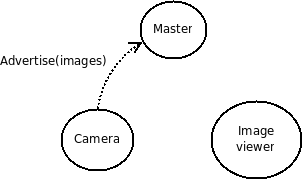
\includegraphics[width=0.30\textwidth]{img/ros_master/ros_master1.png}
    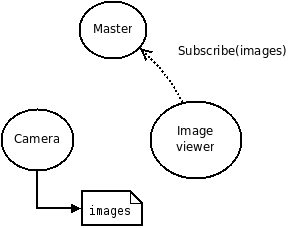
\includegraphics[width=0.30\textwidth]{img/ros_master/ros_master2.png}
    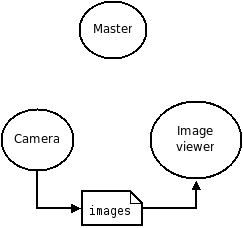
\includegraphics[width=0.30\textwidth]{img/ros_master/ros_master3.png}
    \caption{The process how a camera node informs the ROS-master about the advertisement of information in the images topic and an other image viewer node subscribe to the same topic which leads to a peer-to-peer connection over the images topic.}\label{fig:ros_master}
\end{figure}

The advertisement and subscriptions are managed by the ROS-Master which holds the information to establish the peer-to-peer connection.
The first step to establish a successful connection is the notification of the master about the new topic.
To that moment no data is send, because the topic has no subscriber.
To use the information an other node needs to subscribe to the topic by informing the master about the subscription.
Now the master gives the information to establish a peer-to-peer connection between the nodes and the information goes directly from one node to the other.
Figure \ref{fig:ros_master} visualizes the process with an example how a camera node and image viewer node establish their connection \cite{rosMaster}.

The exchanged information are structured in messages which have predefined structures.
ROS provides messages for the most common usages but they can also be custom made.
Each topic is strongly related to a message type, even if the type is not checked by the ROS-master.

\begin{wrapfigure}[10]{O}{0.4\textwidth}
    \centering
    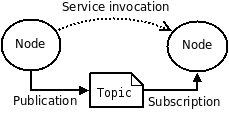
\includegraphics[width=0.4\textwidth]{img/ros_master/service.png}

    \caption{A service invocation is not related to a topic and usually is not a constant flow of messages}
    \label{fig:service_invocation}
\end{wrapfigure}

The publish/subscribe model supports a very flexible way to communicate and can easily scale to big many-to-many models.
But for request/reply situations it is not appropriated.
In these situations services can be used.
They are defined by a pair of messages, one for the request and one for reply.
The call of a service is similar to the connection with a topic except that it is just for the time between the request and the reply.
But nodes can also establish a persistent connection to a service, which causes less robustness but a higher performance.

\subsection{Visualization}\label{ssec:visualization}

In ROS the visualization of data is realized in the tool named \texttt{RVIZ}.
To the user \texttt{RVIZ} itself acts as a host application for different plugins where each message type has it's own plugin.
For ROS \texttt{RVIZ} acts as a normal node so that the individual plugins needs to be configured to subscribe to the relevant topics and how the visualization should look like.

\texttt{RVIZ} provides a number of plugins for the standard messages, but one can also develop their own plugins to visualize the custom messages.

The visualization always happens with respect to one coordinate frame from the data.
To calculate the position of one measurement in the frame of another measurement \texttt{RVIZ} takes a lookup in the \texttt{\textbackslash tf} (transformation) topic which is dedicated to transformations between different frames.

\subsection{Data Recording}\label{ssec:dataRecording}

The ability to record and playback data is a crucial part of ROS.
Since all available data in ROS are exchanged via topics one just needs to subscribe to the topics witch holds the data that should be recorded.
The file format to save the records is typical a bag.
A bag is created with a tool like \texttt{rosbag}.
The tool subscribes to the wanted topics and writes the messages into the bag file, as they come.
After finishing the recording a bag file can be played back with the same tool.
For the rest of the ROS network it behaves like the messages are published by the original nodes, which makes the handling very easy.

To make the process of writing and reading into bag files efficient the messages are not saved as messages but in the same representation as in the network transport layer.
To have the ability to invest \ac{ROS} bags without installing \ac{ROS}, a programmatic API is provided to iterate over the messages in a \ac{ROS} bag \cite{rosBag}.


\section{MATLAB}\label{sec:matlab}
MATLAB stands for Matrix Laboratory and is a computing environment with it's own programming language.
It's originally designed by Cleve Moler to give his students easy access to LINPACK and EISPACK which are Fortran packages to solve Eigensystem and Linear Equation problems.
Later it got rewritten and extended in C from Jack Little and Steve Bangert.
The main extensions where functions, toolboxes and graphics.

Today it is developed and distributed by MathWorks, which is founded by Moler, Little and Bangert.
Over the time the number of toolboxes, tools and features increased.
So did the number of users in universities.

Together with Simulink, which is an other product from MathWorks, MATLAB is used at over 5000 universities and can be termed as the engineers language~\cite{introductionMatlab}.

\subsection{ROS Toolbox}\label{ssec:rosToolbox}
The \ac{ROS} toolbox is the interface to \ac{ROS} for MATLAB and Simulink and provides the possibilities to create nodes and process the messages from a \ac{ROS} network.
It also provides functions to read from \ac{ROS} bags and handling standard message types.

